\documentclass[11pt,a4paper]{article}
\usepackage[T1]{fontenc}
\usepackage{lmodern}
\usepackage[margin=25mm]{geometry}
\usepackage{amsmath,amssymb,amsthm,booktabs,array}
\usepackage{microtype}
\usepackage{tikz}
\usepackage[hidelinks]{hyperref}
\usepackage{url}
\newtheorem{theorem}{Theorem}
\newtheorem{proposition}[theorem]{Proposition}
\newtheorem{lemma}[theorem]{Lemma}
\newtheorem{corollary}[theorem]{Corollary}
\theoremstyle{remark}
\newtheorem{remark}[theorem]{Remark}
\newcommand{\C}{\mathbb C}
\newcommand{\R}{\mathbb R}
\newcommand{\Z}{\mathbb Z}
\newcommand{\pn}[1]{\left\lVert #1\right\rVert_{P}}
\newcommand{\ev}{\operatorname{ev}}
\newcommand{\conv}{\operatorname{conv}}
\newcommand{\code}[1]{\texttt{#1}}
\title{A five-colour lower bound for the\ regular fourteen-gon norm}
\author{Bartosz Paprzycki\\[3pt]\small Independent}
\date{19 October 2026}
\hypersetup{pdftitle={A five-colour lower bound for the regular fourteen-gon norm},pdfauthor={Bartosz Paprzycki}}
\begin{document}
\maketitle
\begin{abstract}
Let $P$ be a regular fourteen-gon centred at the origin. We prove that
every colouring of the plane in four colours has a monochromatic pair
at distance one in the norm whose closed unit ball is $P$.
The proof uses a graph on $1\,540$ labelled vertices with $13\,755$ edges,
realised at unit distance by coordinates in $\Z[e^{\pi i/7}]$.
Exact algebraic witnesses certify every edge, and a propositional
refutation rules out a proper four-colouring of the graph.
The geometric argument, finite obstruction and transfer to the plane
are formalised in Lean. Together with Geh\'er's upper bound, the result
gives $5\leq\chi(\R^2,P)\leq6$.
\end{abstract}

\section{Introduction}

For a centrally symmetric convex body $P\subset\R^2$ with the origin in
its interior, let $\chi(\R^2,P)$ denote the least number of colours needed
to colour the plane so that points at distance one in the norm with
unit ball $P$ receive different colours. No measurability condition is
imposed on the colour classes.

Exoo, Fisher and Ismailescu proved a lower bound of five when the unit
ball is a regular octagon, decagon or dodecagon
\cite{efi}. Their Problem~5.1 asks whether the same lower bound holds
for every regular $2n$-gon with $n\geq4$, and more generally for centrally
symmetric polygons with that many sides. We establish the regular
fourteen-gon case by constructing a finite unit-distance graph with no
proper four-colouring. The construction follows their sumset strategy;
the geometry and colouring obstruction are verified in Lean.

Identify $\R^2$ with $\C$ and set
\[
 \zeta=e^{\pi i/7},\qquad
 P=\conv_{\R}\{1,\zeta,\ldots,\zeta^{13}\},\qquad
 \pn{z}=\inf\{r>0:z\in rP\}.
\]
The set $P$ is a regular fourteen-gon of circumradius one. Changing its
scale or orientation gives an isometric normed plane after the
corresponding linear change of coordinates.

\begin{theorem}\label{thm:main}
For every map $c:\C\to\{0,1,2,3\}$, there are $x,y\in\C$ such that
$\pn{x-y}=1$ and $c(x)=c(y)$. In particular,
$\chi(\R^2,P)\geq5$.
\end{theorem}

Geh\'er proved that six colours suffice for every regular polygon with an
even number of vertices at most $22$ \cite[Theorem~1]{geher}. Thus:
\begin{corollary}\label{cor:bounds}
$5\leq\chi(\R^2,P)\leq6$.
\end{corollary}
We do not determine which of these two values is correct.

The proof combines an exact unit-distance realisation
(Sections~\ref{sec:geometry}--\ref{sec:graph}) with a machine-checkable
refutation of the graph's four-colouring formula (Section~\ref{sec:sat}).
A colouring of the plane would restrict to a colouring of this graph;
Section~\ref{sec:transfer} gives the resulting contradiction.

\section{The polygon norm and its unit sides}\label{sec:geometry}

The set $P$ is compact, convex and symmetric under $z\mapsto-z$, since
$\zeta^7=-1$. The vectors $1$ and $\zeta$ are linearly independent over
$\R$, so $\conv\{1,-1,\zeta,-\zeta\}\subset P$ contains a neighbourhood
of zero. Hence the gauge $\pn{\cdot}$ is finite. Convexity gives the
triangle inequality, symmetry gives absolute homogeneity, and boundedness
gives positive definiteness. Thus this gauge is a norm. Compactness
also gives $\{z:\pn{z}\leq1\}=P$.

The following elementary fact is the geometric part of the edge checker.
\begin{lemma}\label{lem:side}
For $j\in\Z$ and $0\leq t\leq1$,
\[
 \pn{\zeta^j\bigl((1-t)+t\zeta\bigr)}=1.
\]
\end{lemma}
\begin{proof}
Multiplication by $\zeta$ permutes the vertices of $P$, hence preserves
$P$ and its gauge. It is enough to treat $j=0$.
Put $\theta=\pi/7$ and define the real linear functional
\[
 L(z)=\operatorname{Re}z+\operatorname{Re}(\overline\zeta z),\qquad
 h=1+\cos\theta>0.
\]
For a vertex $\zeta^k$,
\[
 L(\zeta^k)=\cos(k\theta)+\cos((k-1)\theta)
 =2\cos(\theta/2)\cos((k-\tfrac12)\theta)\leq h.
\]
The last inequality holds because the angles $(k-\tfrac12)\theta$,
modulo $2\pi$, are at least $\theta/2$ from zero. Equality holds for
$k=0,1$. By convexity, $L(z)\leq h$ for every $z\in P$.

Now $s=(1-t)+t\zeta$ belongs to $P$ and satisfies $L(s)=h$.
Membership gives $\pn{s}\leq1$. If $s=ry$ with $r>0$ and $y\in P$,
then $h=rL(y)\leq rh$, so $r\geq1$. Taking the infimum over all such
$r$ proves $\pn{s}\geq1$.
\end{proof}

\begin{figure}[ht]
\centering
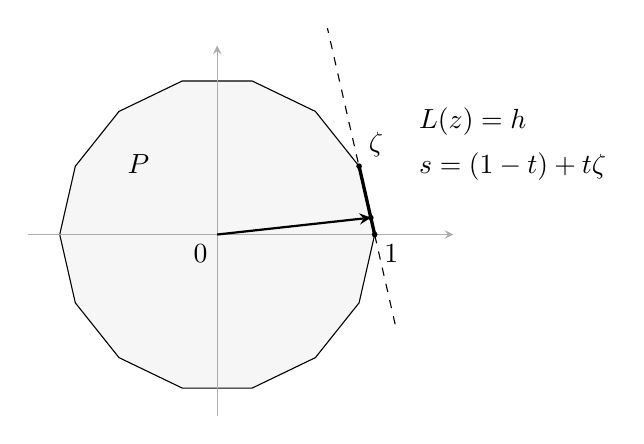
\begin{tikzpicture}[scale=2.0,>=stealth]
 \fill[gray!7] (0:1) \foreach \k in {1,...,13} {-- ({\k*360/14}:1)} -- cycle;
 \draw[thin] (0:1) \foreach \k in {1,...,13} {-- ({\k*360/14}:1)} -- cycle;
 \draw[->,gray!65] (-1.2,0)--(1.5,0);
 \draw[->,gray!65] (0,-1.15)--(0,1.2);
 \draw[very thick] (0:1)--({360/14}:1);
 \draw[dashed] (1.13,-.57)--(.70,1.31);
 \draw[->,thick] (0,0)--(.9755,.1072);
 \fill (1,0) circle(.018) node[below right] {$1$};
 \fill ({360/14}:1) circle(.018) node[above right] {$\zeta$};
 \fill (.9755,.1072) circle(.018);
 \node[anchor=west] at (1.22,.72) {$L(z)=h$};
 \node[anchor=west] at (1.22,.43) {$s=(1-t)+t\zeta$};
 \node at (-.5,.45) {$P$};
 \node[below left] at (0,0) {$0$};
\end{tikzpicture}
\caption{The side from $1$ to $\zeta$ lies on a supporting line of $P$.
Every point on this side has polygon norm one, although its Euclidean
distance from zero need not be one.}
\label{fig:side}
\end{figure}

\section{Exact coordinates for the finite graph}\label{sec:graph}

\subsection{Arithmetic in the cyclotomic coordinates}

For $a=(a_0,\ldots,a_5)\in\Z^6$, write
$\ev(a)=\sum_{k=0}^5a_k\zeta^k$. The identity
\begin{equation}\label{eq:phi}
 \zeta^6-\zeta^5+\zeta^4-\zeta^3+\zeta^2-\zeta+1=0
\end{equation}
follows from $\zeta^7=-1$ and $\zeta\neq-1$.
Consequently multiplication by $\zeta$ can be performed on integer tuples
by the map
\begin{equation}\label{eq:rotate}
 R(a)=(-a_5,\ a_0+a_5,\ a_1-a_5,\ a_2+a_5,\ a_3-a_5,\ a_4+a_5).
\end{equation}
In particular $\ev(R(a))=\zeta\ev(a)$. Subtraction of tuples also
commutes with evaluation.

The side parameters belong to a real cubic field. Set
\[
 \rho=2\cos(2\pi/7)=\zeta^2-\zeta^5.
\]
The second equality views the real number $\rho$ as a complex number.
Reduction using~\eqref{eq:phi} gives
\begin{equation}\label{eq:cubic}
 f(\rho)=0,\qquad f(X)=X^3+X^2-2X-1.
\end{equation}
Moreover $\rho>1$, because $2\pi/7<\pi/3$.
The polynomial $f$ is strictly increasing on $[1,\infty)$:
$f'(X)=3X^2+2X-2>0$ there.
Exact substitution into $f$ yields $f(\ell)<0<f(u)$ for
\begin{equation}\label{eq:interval}
 \ell=\frac{1246979603717467}{10^{15}},\qquad
 u=\frac{1246979603717468}{10^{15}}.
\end{equation}
It follows that $\ell<\rho<u$. This argument identifies the intended
root of~\eqref{eq:cubic} from its geometric definition.

For integers $A,B,C$, let $t=A+B\rho+C\rho^2$. A tuple representing the
point $(1-t)+t\zeta$ is
\begin{equation}\label{eq:side-coordinate}
 S(A,B,C)=(1+B-A-2C,\ A+2C-B,\ 0,\ C,\ B-2C,\ C).
\end{equation}
Indeed, substituting $\rho=\zeta^2-\zeta^5$ and reducing
by~\eqref{eq:phi} gives
$\ev(S(A,B,C))=(1-t)+t\zeta$.

\subsection{The coordinate and witness lists}

Let $V=\{0,\ldots,1539\}$. The coordinate list in the accompanying
file \path{minkowski14_final_graph.json} assigns a tuple $a_v\in\Z^6$ to each $v\in V$;
put $p_v=\ev(a_v)$. Its edge list defines a graph $G=(V,E)$ with
$|E|=13\,755$. Vertex labels are zero based. The files are described in
Appendix~\ref{app:data}, and the complete formal sources are available
in the repository~\cite{artifact}.

For each listed edge $(v,w)$ there is a witness $(j,r)$, where
$0\leq j<14$ and $r$ indexes one of the $29$ triples in
Table~\ref{tab:parameters}. The witness asserts the integer equality
\begin{equation}\label{eq:witness}
 a_v-a_w=R^j(S(A_r,B_r,C_r)).
\end{equation}
Thus verification of an edge reduces to six integer equalities and an
interval bound for $t_r=A_r+B_r\rho+C_r\rho^2$.

\begin{table}[ht]
\centering
\small
\setlength{\tabcolsep}{9pt}
\begin{tabular}{r rrr @ {\qquad} r rrr @ {\qquad} r rrr}
\toprule
$r$&$A_r$&$B_r$&$C_r$&$r$&$A_r$&$B_r$&$C_r$&$r$&$A_r$&$B_r$&$C_r$\\
\midrule
0&-4&0&3&10&-1&1&0&20&2&-1&0\\
1&-4&1&2&11&0&-2&2&21&2&0&-1\\
2&-3&-1&3&12&0&-1&1&22&2&1&-2\\
3&-3&0&2&13&0&2&-1&23&3&-1&-1\\
4&-2&-3&4&14&0&3&-2&24&3&2&-3\\
5&-2&-2&3&15&1&-3&2&25&3&3&-4\\
6&-2&1&1&16&1&-2&1&26&4&0&-2\\
7&-2&2&0&17&1&0&0&27&4&1&-3\\
8&-1&-1&2&18&1&1&-1&28&4&2&-4\\
9&-1&0&1&19&1&2&-2&&&&\\
\bottomrule
\end{tabular}
\caption{The triples used to certify the edges, with the same indices
as in the formal development. Each gives $0\leq t_r\leq1$.}
\label{tab:parameters}
\end{table}

\begin{samepage}
\begin{lemma}\label{lem:parameters}
For each triple in Table~\ref{tab:parameters},
$0\leq A_r+B_r\rho+C_r\rho^2\leq1$.
\end{lemma}
\begin{proof}
Since $0<\ell<\rho<u$, a lower and upper bound for any such expression are
\begin{align*}
 L_r&=A_r+\min(B_r\ell,B_ru)+\min(C_r\ell^2,C_ru^2),\\
 U_r&=A_r+\max(B_r\ell,B_ru)+\max(C_r\ell^2,C_ru^2).
\end{align*}
Substitution of the $29$ triples gives $L_r\geq0$ and $U_r\leq1$.
These are rational inequalities with the fixed denominator $10^{30}$
after clearing fractions. The formal theorem \code{parameter\_bounds}
checks all cases using~\eqref{eq:interval}.
\end{proof}
\end{samepage}

\begin{samepage}
\begin{proposition}[Certified edge list]\label{prop:edges}
Every $(v,w)\in E$ satisfies $\pn{p_v-p_w}=1$.
\end{proposition}
\begin{proof}
The certificate check verifies that every $(v,w)\in E$ has a witness
$(j,r)$ satisfying~\eqref{eq:witness}. This is a finite check of six
integer equalities per edge. Evaluating these equalities gives
\[
 p_v-p_w=\zeta^j\bigl((1-t_r)+t_r\zeta\bigr).
\]
Apply Lemmas~\ref{lem:parameters} and~\ref{lem:side}.
\end{proof}
\end{samepage}

For example, the edge $(0,106)$ has
\[
 a_0=(-6,4,0,1,-4,1),\qquad a_{106}=(-3,2,0,1,-3,1).
\]
Its witness is $j=7$, $r=10$, so $t_r=\rho-1$ and
$S(-1,1,0)=(3,-2,0,0,1,0)$.
Since $\zeta^7=-1$, equality~\eqref{eq:witness} gives
$p_0-p_{106}=-((2-\rho)+(\rho-1)\zeta)$.
The interval~\eqref{eq:interval} puts $\rho-1$ strictly between zero and
one, so this edge corresponds to a point in the interior of a polygon
side, rather than to a polygon vertex.

\subsection{How the witness was obtained}

Following the sumset strategy of Exoo, Fisher and Ismailescu~\cite{efi},
the search used the side parameters
\[
 T=\{0,\rho-1,\rho^2-\rho,\rho^2-1,1+\rho-\rho^2\}.
\]
Each parameter lies in $\Z[\rho]\cap[0,1]$, as follows from
\eqref{eq:interval}. Thus the generating set
\[
 U=\{\zeta^j((1-t)+t\zeta):t\in T,\ 0\leq j<14\}
\]
consists of unit vectors with exact integer-tuple coordinates given by
\eqref{eq:side-coordinate} and~\eqref{eq:rotate}. Forming $U+U$ and
testing differences can therefore be done in the same exact arithmetic.
The search retained unit-distance edges and used unsatisfiable SAT cores
to reduce the graph to the supplied coordinate and edge lists.

\section{The four-colouring obstruction}\label{sec:sat}

For $v\in V$ and $c\in\{0,1,2,3\}$, introduce a Boolean variable
$x_{v,c}$ meaning that vertex $v$ has colour $c$.
Let $F_G$ be the conjunction of the following clauses:
\begin{align}
 &x_{v,0}\vee x_{v,1}\vee x_{v,2}\vee x_{v,3}
 &&(v\in V),\label{eq:atleast}\\
 &\neg x_{v,c}\vee\neg x_{v,d}
 &&(v\in V,\ 0\leq c<d\leq3),\label{eq:atmost}\\
 &\neg x_{v,c}\vee\neg x_{w,c}
 &&((v,w)\in E,\ 0\leq c\leq3),\label{eq:edge-clause}\\
 &x_{759,0}.&&\label{eq:anchor}
\end{align}
There are $4|V|=6\,160$ variables and
\[
 |V|+6|V|+4|E|+1=1\,540+9\,240+55\,020+1=65\,801
\]
clauses. In DIMACS notation, $x_{v,c}$ has index $4v+c+1$;
the last clause is therefore \code{3037 0}.

\begin{lemma}\label{lem:encoding}
If $G$ has a proper four-colouring, then $F_G$ is satisfiable.
\end{lemma}
\begin{proof}
Permute the four colour names so that vertex $759$ has colour zero.
Assign $x_{v,c}$ to be true precisely for the assigned colour of $v$.
Clauses~\eqref{eq:atleast} and~\eqref{eq:atmost} express that each vertex
has exactly one colour, clauses~\eqref{eq:edge-clause} hold by properness,
and~\eqref{eq:anchor} holds by the permutation.
\end{proof}

\begin{proposition}[Certified refutation]\label{prop:unsat}
The formula $F_G$ is unsatisfiable. Consequently $G$ has no proper
four-colouring.
\end{proposition}
\begin{proof}[Computer-assisted proof]
The file \path{minkowski14_final_4color.lrat.gz} contains an LRAT refutation of the
exact formula in \path{minkowski14_final_4color.cnf}. LRAT is a clausal proof format
that supplies hints for checking each added clause~\cite{lrat}.
The trace is imported in $42$ parts as ordinary Lean proof expressions;
the final part derives the empty clause. The formal encoding theorems
identify the imported formula with the clauses
\eqref{eq:atleast}--\eqref{eq:anchor}, including the anchor condition.
Lean checks both this identification and the refutation. Hence $F_G$
is unsatisfiable, and Lemma~\ref{lem:encoding} rules out a proper
four-colouring of $G$.
\end{proof}

The supplied trace allows this derivation to be checked independently
of the search and the SAT solver.

\section{Transfer to the plane}\label{sec:transfer}

\begin{proof}[Proof of Theorem~\ref{thm:main}]
Suppose that $c:\C\to\{0,1,2,3\}$ assigns different colours to every
pair at polygon distance one. Colour each vertex $v$ of $G$ by $c(p_v)$.
Proposition~\ref{prop:edges} makes this a proper four-colouring of $G$,
contradicting Proposition~\ref{prop:unsat}.
\end{proof}

The listed edges suffice for the contradiction, even if other pairs
among the coordinates also have unit distance. The pullback colouring
is well defined even when two vertex labels represent the same point;
adjacent vertices have distinct images because their distance is one.
A colouring with fewer than four colours also gives a map to
$\{0,1,2,3\}$, so the argument rules out all such colourings.

\section{Formalisation and reproducibility}\label{sec:formal}

The formalisation uses Lean~4.34.0 and mathlib at commit
\begin{center}\small\code{5ed2965256430c3649e86755f9576b54eca72435}.\end{center}
The type \code{Minkowski14.Plane} is the complex plane equipped with the
polygon norm. Theorems \code{plane\_dimension}, \code{plane\_unit\_ball}
and \code{plane\_distance} establish, respectively, its real dimension
two, its closed unit ball $P$, and its distance function
$d(x,y)=\pn{x-y}$. These theorems identify the formal normed space with
the geometric plane used in Theorem~\ref{thm:main}.

The final theorem, \code{Minkowski14.at\_least\_five\_colours}, states
that for every natural number $n$ and every map $c$ from this plane to
\code{Fin n}, the hypothesis
\[
 \forall x,y,\quad d(x,y)=1\ \Longrightarrow\ c(x)\neq c(y)
\]
implies $5\leq n$. Here \code{Fin n} is the type of natural numbers
strictly less than $n$.

\begin{table}[ht]
\centering\small
\begin{tabular}{>{\raggedright\arraybackslash}p{.40\linewidth}>{\raggedright\arraybackslash}p{.51\linewidth}}
\toprule
Mathematical component & Formal sources under \code{formal/}\\
\midrule
Polygon norm and supporting side & \code{Polygon.lean}, \code{Facet.lean}\\
Cyclotomic arithmetic and parameter bounds & \code{Algebra.lean}, \code{Coordinates.lean}, \code{Parameters.lean}\\
Coordinate and edge certificates & \code{Positions.lean}, \code{Geometry/}, \code{Embedding.lean}\\
Colouring formula and refutation & \code{MathIsEasy/Minkowski14/}, \code{MathIsEasy/Minkowski14LRAT/}\\
Normed plane and final transfer & \code{Plane.lean}, \code{ColouringTransfer.lean}, \code{Final.lean}\\
\bottomrule
\end{tabular}
\caption{Where to compare the mathematical statements with their formal versions.}
\label{tab:formal}
\end{table}

A public build on 6 October 2026 compiled all $162$ project modules
from source and rejected three deliberately invalid controls: a false
coordinate equality, a false SAT refutation, and a proof expression of
the wrong type. A valid small SAT control passed. The source files are
matched to the compiler records by SHA-256 hashes.

The final theorem depends only on the standard Lean axioms
\code{propext}, \code{Classical.choice} and \code{Quot.sound}.
The project proof has no additional axioms, admissions, \code{unsafe}
declarations or uses of \code{native\_decide}. Proof expressions are
checked by Lean's ordinary kernel. This verification relies on the
kernel and the correspondence between the formal and mathematical
statements. No separate kernel implementation was used.

The repository includes the pinned dependencies, build procedure,
compiler records, axiom output and failed-control diagnostics~\cite{artifact}.
Its lightweight integrity command checks hashes and correspondence of
the published files without compiling Lean. Rebuilding the proof is
a separate operation, described in \code{REPRODUCE.rst}.

\section{Further questions}

Does the entire plane admit a
proper five-colouring? How small can a finite unit-distance obstruction
to four colours be? Extending the construction to
other regular polygons would address further cases of
\cite[Problem~5.1]{efi}; the coordinates and side parameters used here
are specific to the fourteen-gon.

\section*{Use of AI}

The author initiated and directed this work but has no background
in mathematical research and did not supply the mathematical argument.
The graph search, certificate generation, geometric proof, Lean
formalisation and manuscript were developed with AI assistance.
OpenAI Codex (GPT-6 Astra) was used for the complete geometric
formalisation, verification tools and exposition.
Independent human peer review of the manuscript is not claimed.

\section*{Acknowledgements}

The author thanks Panna Geh\'er and Dan Ismailescu for correspondence
about the problem and suggestions for further work.
The project was inspired by the YouTube channel \code{@xamualexander},
Dr.~Samuel Allen Alexander. Still there.

\appendix
\section{Data files and certificate conventions}\label{app:data}

The data files are included in the repository~\cite{artifact}.
The graph, colouring formula and LRAT certificate are under
\code{formal/artifacts/}; the edge witnesses are in \code{docs/graph.json}.
\begin{description}
\item[\path{minkowski14_final_graph.json}]\hfill\\
The exact coordinate and edge lists.
The field \code{vertices\_power\_basis} contains the six integers
$(a_0,\ldots,a_5)$ for each vertex, in label order. The field \code{edges}
contains pairs of zero-based vertex labels. Only these two fields define
the graph used in the proof.
\item[\code{docs/graph.json}]\hfill\\
The same coordinates, the ordered
parameter triples, and triples $(v,w,k)$ for the edges. Decode a witness
by $r=\lfloor k/14\rfloor$ and $j=k\bmod14$, then check
\eqref{eq:witness}. Edge order may differ from \path{minkowski14_final_graph.json}; the
edge sets agree.
\item[\path{minkowski14_final_4color.cnf}]\hfill\\
The DIMACS formula described in
Section~\ref{sec:sat}.
\item[\path{minkowski14_final_4color.lrat.gz}]\hfill\\
The gzip-compressed LRAT refutation;
decompress it before replay. Its filename in the Lean project is
\path{minkowski14_final_4color.lrat}.
\item[\code{formal/}]\hfill\\
The complete Lean sources and pinned dependencies.
The repository's \code{REPRODUCE.rst} gives the build instructions;
precompiled project results are not required.
\item[\code{evidence/}]\hfill\\
Source and certificate hashes, compiler records,
axiom output and control results.
\end{description}

For comparison with the recorded build, the SHA-256 hash of the
\emph{decompressed} LRAT file is
\begin{center}\small\ttfamily
9ff6788806bedd8596fb8972fa546d86b6e193dc950e2542a2dcc4e29b27b2d6
\end{center}

\begin{thebibliography}{9}
\raggedright
\bibitem{efi}
G.~Exoo, D.~Fisher and D.~Ismailescu,
\emph{The chromatic number of the Minkowski plane---the regular polygon case},
2021. \href{https://arxiv.org/abs/2108.12861}{arXiv:2108.12861}.

\bibitem{geher}
P.~Geh\'er,
\emph{Note on the chromatic number of Minkowski planes: the regular polygon case},
2023. \href{https://arxiv.org/abs/2301.13695}{arXiv:2301.13695}.

\bibitem{lrat}
L.~Cruz-Filipe, M.~J.~H.~Heule, W.~A.~Hunt Jr., M.~Kaufmann and
P.~Schneider-Kamp,
\emph{Efficient certified RAT verification},
2016. \href{https://arxiv.org/abs/1612.02353}{arXiv:1612.02353}.

\bibitem{artifact}
B.~Paprzycki (MathIsEvenEasier),
\emph{Minkowski fourteen-gon: graph, certificates and Lean formalisation},
2026. \url{https://github.com/MathIsEvenEasier/minkowski14}.
The recorded public source build uses commit
\code{e0f5e2a086fb0ab080b4a9393b72d33fc87e5918};
\href{https://github.com/MathIsEvenEasier/minkowski14/actions/runs/37468510724}{build and compiler records}.
\end{thebibliography}
\end{document}
